\chapter{A Conceptual Framework for Information Discovery and Curation on the Web}
\label{chapter:framework}

Although Web-based information discovery and curation tasks are commonly performed today, as we mentioned above, there is a lack of literature on how to enable and support them when building Web applications. I reduce this gap by presenting a framework of design factors facilitating digital information discovery and curation. 

In my framework, I built on existing models and frameworks of information discovery and curation and analysis of existing Web tools to derive corresponding design factors for Web design. I borrow terminology from Activity Theory~\cite{kuutti1996activity} to describe how different components of the framework are connected. 

The framework is divided into two parts. This chapter outlines the first part of the framework titled \textit{``Enabling Information Discovery and Curation''}. The first part of the framework consists of motives behind information discovery and curation, actions that discovery and curation consist of, and design factors that enable those actions (see Figure~\ref{fig:framework_part1}). Second part of the framework deals with improving operations that are involved in information discovery and curation (see Chapter~\ref{chapter:improving}).

\begin{figure}[ht!]
	\noindent
	\centering
	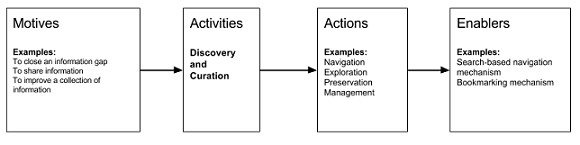
\includegraphics[width=\linewidth]{framework_part1.png}
	\caption{Framework Overview (Part I): Enabling Information Discovery and Curation}
	\label{fig:framework_part1} 
\end{figure}

{\section{Motives Behind Information Discovery and \\ Curation}
Understanding the motives behind user activities can help form a conceptual model of a needed Web application and its features. There exists a wide variety of user motives behind information discovery and curation, and certain aspects of these motives can significantly impact the design of an application. The following generalizations of motives and their properties can help define conceptual models and identify primary use cases of Web tools for information discovery and curation.  

{\subsection{Closing Knowledge Gap}
The primary motive for information discovery is usually to close a knowledge gap that occurs when the user tries to accomplish a task and lacks information to do so. This motive can take up various forms. Its form commonly depends on the nature of an information need and other conditions surrounding the given motive.        

Depending on the context in which it arose, an information need can have various degrees of specificity. For example, if the motive is to find inspiration for a project, an information need is only vaguely defined. However, if the motive is to find a phone number of a specific business, an information need is well-defined. In some cases, the information need may be hidden, and the user might not be aware of the existing knowledge gap. The specificity of an information need determines important properties of information discovery mechanisms, such as whether users can benefit more from mechanisms that allow to specify an information need, help form an information need, or allow to randomly retrieve information. This property has to be taken into consideration when evaluating or designing a Web application. 

The nature of an information need predetermines whether discovery is respectively serendipitous or oriented towards fact finding. Therefore, depending on user needs, an application can be designed to increase serendipity and opportunistic discovery or to improve purposeful fact finding. For instance, displaying featured content can improve serendipitous discovery because of its inconsistent nature and novelty. Using context, such as location and date, to tailor search results to the user can improve fact finding. 

The motive behind information rediscovery involves finding previously discovered information and closing previously closed knowledge gap in case if information was forgotten. It usually results in the user looking for previously found resources and Web pages. In fact, Web-page revisitation is one of the most commonly performed web-browsing activities~\cite{adar2008large,cockburn2003improving}. The percentage of revisited web pages involved in web browsing can range from 58\%~\cite{tauscher1997people} to 81\%~\cite{cockburn2001web}. Some of the reasons for revisiting pages include shopping, communication, entertainment, education, activity planning, and hobby-related information retrieval~\cite{adar2008large}. Some Web pages and resources can be rediscovered using navigation while others need to be previously preserved (bookmarked) in order to allow rediscovery. Rediscovery is one of the many ways in which information discovery and curation interweave. 

Another type of motive for information discovery relates to the two qualities of the Web defined by Lindley et al. - temporality and persistence~\citep{lindley2012s}. \textit{Persistence} refers to the quality of the Web that allows people to habitually revisit Web pages and continue on-going Web projects. \textit{Temporality} refers to the quality of the Web that allows the content of websites to be continuously updated to provide users with new information. Persistence alone usually facilitates information rediscovery. However, if persisitence is combined with temporality, they can facilitate discovery of new information within the same application or channel. I refer to this type of discovery as \textit{channel-based discovery}. Some of the common motives for channel-based discovery include orienting (or monitoring for updates) and opportunistic information discovery~\citep{lindley2012s}.          
}

{\subsection{Future Use and Reaccess}
The main motive behind information curation is to make it possible to retrieve information and to consequently use it. In order to facilitate easy information retrieval, many Web applications employ various forms of bookmarking systems. Traditionally, bookmarks are manually organized by users into folders. However, this method of organization has been found inefficient because folders with bookmarks become easily cluttered~\cite{abrams1998information}. Therefore, in order to efficiently support information rediscovery, Web tools need to provide mechanisms for information preservation along with information management.
}

{\subsection{Improving Collection}
Reportedly, people gather information to improve existing collections~\cite{lindley2012s}. Although some deeper motives may include self reflection or the possibility of future use, collecting information is a motive in itself. In general, information gathering may be stretched over a period of time~\cite{kellar2006goal}, resulting in repeating page visitation. Although information gathering composes only 13.4\% of Web usage, it highly contributes to various goal-supporting activities, such as decision making and planning~\cite{kellar2006goal}.

}

{\subsection{Communication}
As part of his information behavior model, Wilson identified communication of information as an outcome of information seeking. Communication can also be thought of as a motive for information discovery and curation. To support communication of information, Web tools have to provide mechanism that allow various users to share information among themselves. 

In recent years, social bookmarking, a way to preserve and share information within various communities, has gained popularity as an effective way of communicating with other users~\cite{estelles2010social}. One of the first visions of social bookmarking was associated with Web blogging. Oravec~\cite{oravec2002bookmarking} believes that web blogs help annotate or bookmark important information and build a ``map'' of the Internet. Evolution of social bookmarking has advanced bookmarking technologies and provided a means for collaborative information discovery and curation. 
}

Even though it is not entirely feasible to list all of the possible motives for information discovery and curation, in this section I outline some of the important motives and their aspects that can aid in developing use cases and formalizing conceptual models for Web applications. These motives also make it easier to showcase how mechanisms for discovery and curation complement each other. 
}

{\section{Discovery and Curation Activities, Actions, and Their Enablers}
The next portion of the framework consists of two main categories (discovery and curation) that are consequently decomposed into different actions (see Figure~\ref{fig:enablers}). Each of the actions is supported by a group of features or mechanisms that enable given aspect of discovery or curation in a Web application.  The following subsections describe each of the groups and outline corresponding questions that can help application design and evaluation.  

\begin{figure}[ht!]
	\noindent
	\centering
	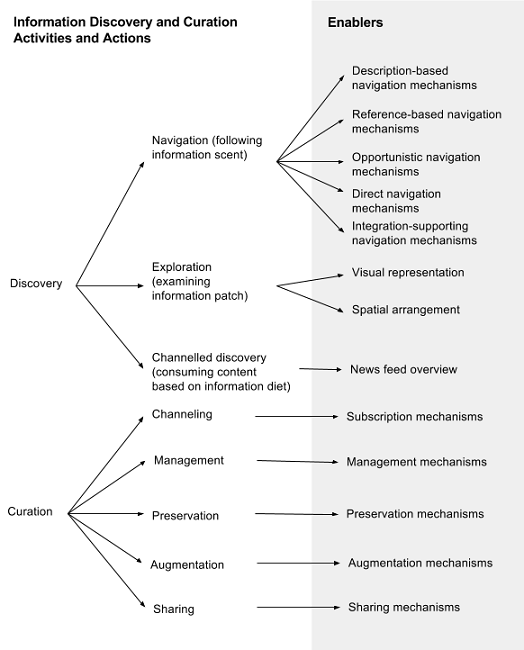
\includegraphics[width=\linewidth]{framework_enablers.png}
	\caption{Enabling Information Discovery and Curation: Activities, Actions, and Corresponding Enablers}
	\label{fig:enablers} 
\end{figure}

{\subsection{Navigation in Discovery: Following Information Scent}
In order to discover information, a user needs to have a way of navigating to it. Navigation in information discovery can be thought of as following an information scent. In general, information scent models deal with how the users identify value, cost, or access path of information sources based on proximal cues, such as links, icons, categories, etc.~\cite{pirolli1999information}. Common methods of navigation that facilitate information discovery include descriptional, referential, opportunistic, and system-regulated (see Table~\ref{table:navigation}). 


\begin{table}[ht!]
\caption{Navigation Mechanisms}
\label{table:navigation} 
\begin{tabular}{{|p{0.33\linewidth}|p{0.67\linewidth}|}}
\hline
Navigation mechanisms     	& Questions to be posed during the design or evaluation of  discovery and curation tools \\
\hline
\textbf{Descriptional} 			& \\
Search-based navigation							& Is it possible to navigate within the application using a search mechanism? \\
Integrated search				& Is it possible to retrieve information from  other applications using a search mechanism? \\
\textbf{Referential}       		& \\
Categories				 		& Is it possible to navigate using categories? \\
Facets				    		& Is it possible to navigate using facets? \\
Filters					  		& Is it possible to navigate using filters? \\
Tags				      		& Is it possible to navigate using filters? \\
Search by item or resource		& Is it possible to search by item or resource? \\
Integrated reference			& Is it possible to retrieve information from other applications using any of the referential mechanisms?\\
\textbf{Opportunistic}          & \\
Opportunistic navigation        & Is it possible to opportunistically navigate through information within the application? \\
Integrated opportunistic navigation        & Is it possible to opportunistically retrieve information from other application? \\
\textbf{System-regulated}            		& \\
Static direct display           & Is it possible to view static information directly without active search? \\
Integrated static display   	& Is it possible to view static information from other applications without active search? \\
Featured content             	& Is it possible to view featured content? \\
Integrated featured content     & Is it possible to view featured content from other applications? \\
News feed             			& Is it possible to view news feed? \\
Integrated news feed            & Is it possible to view news feed from other applications? \\
\hline
\end{tabular}
\end{table}

{\subsubsection{Descriptional Navigation}
A navigation is descriptional when the user has a means of describing their information need. Most commonly it is implemented as search-based navigation since it allows users to enter the search query and describe what they want to find. Some of the modern descriptional navigation systems can be activated using voice. 

Almost every present-day Web application has the search feature implemented, with rare exceptions of applications that utilize other methods of navigation, such as StumbleUpon and certain shopping websites. Some Web applications are integrated with others enabling users to search multiple websites at once.    

There exist numerous ways in which descriptional navigation supports information discovery. Search-based navigation often serves as an entry point for information seeking~\cite{levene2011introduction}. When the motive behind information discovery has a well-articulated information need, then the user can express their information need by entering a search query. 

Descriptional navigation can also help to rediscover information. However, it is not always a reliable way of refinding information ~\cite{cockburn2003improving}. In information portals that provide access to fairly ambiguous information and that have regularly updated information flow, the search feature is usually designed around retrieving information related to some general topic. In order to make search-based navigation a reliable way to rediscover information, it must return consistent results. 
} % end subsection

{\subsubsection{Referential Navigation}
A navigation is referential when the user finds a reference, such as link or icon, to the term that they are looking for. This reference represents an information scent. The underlying assumption of this method of navigation is that the user can recognize needed information or a reference to it as they see it~\cite{waterworth1991model}. 

Referential navigation mechanisms can take many different forms. Some common types are categories, facets, filters, and tags. In some applications, users can search by a given resource. For example, YouTube provides a playlist with music related to the currently playing song. Information scent representatives may also reference sources outside of the given system. This enables another type of integration of Web applications. 

Referential navigation can help the user identify their information need by suggesting terms, topics, or categories to use, and therefore, directing the user to relevant resources~\cite{levene2011introduction}. It can also help narrow the results to a specific type of resource so that further discovery is bounded by that type. For example, TripAdvisor allows the user to choose among hotels, flights, vacation rentals, restaurants, and destinations, so the application helps to narrow search results.

} % end subsection

{\subsubsection{Opportunistic Navigation}
Opportunistic navigation is method of navigating ``randomly" though resources and Web pages.  As expected, this type of navigation is not authentically random; therefore, I apply the term ``opportunistic" to describe this type. However to the user, this navigation type appears to be randomized, and it promotes serendipitous discovery. This method is especially useful when the information need is fully undefined.

Many applications, such as StumbleUpon and Wikipedia, support opportunistic navigation to allow for opportunistic jumping from one resource to another. StumbleUpon makes it possible to explore the Web in general - other websites and Web applications, allowing for integrated navigation, whereas Wikipedia provides opportunistic access to its own articles. 
} % end subsection

{\subsubsection{System-regulated Navigation}
Often, Web applications display or update information without the user's active participation. This information can be news feed, featured deals or articles, static information, or other types of content. In my thesis, I refer to this type of navigation as system-regulated because it occurs when the application brings the content to the user instead of the user applying any effort to find it. It differs from opportunistic navigation because the the user cannot choose when to observe new information; instead, all updates are regulated by the application. 

One example of an application that utilizes system-regulated navigation is Yelp. This tool displays featured restaurants as well as its user's recent activities as soon as the user enters the site. As any other navigation method, this method can ensure cross-application integration by displaying content from other Web applications. 
} % end subsection
} % end section

{\subsection{Exploration and Discovery}
Exploration of resources is another factor that enables information discovery. In particular, visual and spatial explorations of single or multiple resources allow for rapid information searching (see Table ~\ref{table:exploration}). 

Abrams et al.~\cite{abrams} identified link representation as one of the problems with traditional bookmarking. Analogous with browsing through a bookmark manager, identifying relevant information when browsing through links to diverse resources can be a challenging task. A visual preview should make it easier to evaluate the relevance of resources. Applications that facilitate serendipitous information discovery often employ elaborate resource representation techniques. Many social bookmarking systems, such as Scoop.it! and StumbleUpon, support visual previews of bookmarked pages. Delicious is a social bookmarking application that lacks this type of link representation support, which makes it harder to determine if the link will lead to a relevant resource.

Similar to link representation, spatial visualization of numerous links is another problem that occurs when browsing through diverse content ~\cite{abrams}. Therefore, a semantic to the spatial arrangement of resources is of major importance. Information discovery applications that support serendipitous discovery often have a special way of spatially arranging resources to make it easier to browse through large amounts of information. For example, many tools use a 'pinboard' layout of resources similar to Pinterest.

\textbf{Uniform representation.} Uniform representation is a method of displaying diverse resources in a common way, with each resource having the same set of components ~\cite{herrera}. Such a representation assures that each resource has the same set of facts associated with it, and therefore, the user can afford to have expectations about information that can be found when looking for a specific fact. For example, Yelp displays rating, price range, and address for all restaurants, so not only is it easy to find specific information, but the user can have expectations about the content of resources within the application. On the contrary, searching Tumblr for a restaurant will return a chaotic collection of information about the place. 



\textbf{Visual link preview.} If an application provides links to resources, a visual preview makes it easier to recognize the relevance of the resource ~\cite{abrams}. Applications that support fact discovery often use visual link preview, similar to applications that support serendipitous browsing. However, the motivation behind having a link preview for fact finding is to make it possible to identify if the resource is indeed what the user is looking for. For example, searching for an actor in IMDb will return a list of actors and their photographs, so that the user can pick the one they are interested in.

\textbf{Spatial arrangement.} Similar to serendipitous information discovery, spatial arrangement of resources is important ~\cite{abrams} as a poor semantic to the arrangement can make it difficult to visually navigate to the facts of interest.

\begin{table}[ht!]
\caption{Visual and Spatial Exploration Mechanisms}
\begin{tabular}{{|p{0.33\linewidth}|p{0.62\linewidth}|}}
\hline
Exploration mechanisms & Questions to be posed during the design or evaluation of discovery and curation tools  \\
\hline
\textbf{Visual and textual cues of multiple resources} & \\
Visual preview  & Are there visual previews of resources to help identify resources of value? \\
Textual preview & Are there textual previews of resources to help identify resources of value? \\
\textbf{Visual and textual cues of a single resource} & \\
Visual cues                 & Are there visual cues to help identify the value of information within a resource? \\
Textual cues                & Are there textual cues to help identify the value of information within a resource? \\
\textbf{Spatial proximal cues of multiple resources} & \\
List  						& Are resources presented in a list? \\
Grid   						& Are resources presented in a grid? \\
Gallery  					& Are resources presented in a gallery layout? \\
Spatial semantic            & Is there a semantic to the spatial arrangement of multiple resources? \\ 
Consistency				 	& Are resources presented in a consistent way? \\                                                    
\textbf{Spatial proximal cues of a single resource} & \\
Spatial semantic            & Is there a semantic to the spatial arrangement of information within a resource? \\
Consistency   				& Are same types of resources presented in a consistent way?\\                                                       
\hline
\end{tabular}
\end{table}


} % end section
{\subsection{Integration}

Similar to serendipitous discovery, if an information discovery application provides access to resources from other Websites, the user should be able to navigate to those sites as they may contain the facts of interest. Integration for fact finding is especially important when it gives an opportunity to display specific information about resources that otherwise would not be accessible. For example, Google Maps displays business ratings as a result of its integration with Google+.

To users with ambiguous information needs, one information portal might not provide access to all information of interest. If an information discovery application gives access to resources from various sources, such as other Websites, the user should be able to navigate back to those sources.  
} % end section

{\subsection{Curation}

Information curation is a common activity within many information discovery applications. By asking questions about application design with regards to information curation as in Tables~\ref{table:curation} and~\ref{table:curation_support} of the conceptual framework, designers can find ways to add value to information and enable information exploitation over time.

Information discovery applications vary from being completely socially curated and populated by users, to those that lack any curation mechanisms. 
By definition, digital information curation is the notion of managing, preserving, and adding value to collections of information ~\cite{beagrie, wittaker}. Thus, the curation category consists of information management, preservation, information enhancement, and sharing.


\begin{table}[ht!]
\caption{Curation Mechanisms}
\label{table:curation}
\begin{tabular}{{|p{0.30\linewidth}|p{0.65\linewidth}|}}
\hline
Curation mechanisms  & Questions to be posed during the design or evaluation of  discovery and curation tools  \\
\hline
\textbf{Management} & \\
Collection-based categorization     & Is it possible to sort information into collection-like structures, either privately or publicly? \\
Tag-based categorization          	& Is it possible to tag information, either privately or publicly? \\
\textbf{Preservation} & \\
Internal preservation of internal resources		& Is it possible to preserve internal information within the application? \\
Internal preservation of external resources     & Is it possible to preserve external information within the application? \\
External preservation of internal resources     & Is it possible to preserve internal information outside of the application? \\ 
\textbf{Augmentation} & \\
Annotation & Is it possible to annotate resources, either privately or publicly? \\ 
Evaluation & Is it possible to evaluate resources, either privately or publicly? \\       
\textbf{Sharing} & \\
Adding resources        & Is it possible to add resources to the collection of information within the application from other websites? \\
Internal sharing        & Is it possible to publicly reshare internal resources within the application? \\ 
External sharing        & Is it possible to publicly reshare internal resources outside of the application? \\ 
\textbf{Channel-picking}  	& \\
User subscription       & Is it possible to subscribe to activities of other users? \\
Site subscription       & Is it possible to subscribe to site updates? \\
Artifact subscription  	& Is it possible to subscribe to artifact updates?\\
\hline        
\end{tabular}
\end{table}




{\subsubsection{Management}
Information management is one of the key elements of information curation ~\cite{beagrie, wittaker}. Information categorization mechanisms are prevalent in applications that have a lot of information that is hard to categorize automatically or can mean something different for each user. In the context of Web information management, the following factors play a major role.

Resource categorization helps establish relationships between various resources ~\cite{beagrie, wittaker}. Allowing people to sort information using custom categories can aid rediscovery, discovery in a socially curated space, as well as add more value to resources.

Similar to list-based categorization, tagging aids rediscovery, adds value to resources, and aids discovery, especially in a socially curated space ~\cite{gruber}.  For example, Pinterest supports tag- and list-based categorizations, where lists are represented as 'pinboards'. Tumblr, on the other hand, only supports tag-based categorization. In addition, Pinterest allows for private information categorization.

} % end subsubsection

{\subsubsection{Information Preservation}
Information preservation is a common Web task that is usually performed with the intent of revisiting information ~\cite{abrams, wittaker}. However, in the case of opportunistic Web use, information gathering is sometimes performed with just the goal of collecting information rather than revisiting it in the future ~\cite{lindley}. Bookmarking is a traditional way of preserving information and many Web applications provide diverse bookmarking mechanisms. 

Internal preservation of internal resources means bookmarking resources to be reaccessed within the same application. Such bookmarking facilitates information curation within the system.

Internal preservation of external resources signifies bookmarking other Web pages within an application. 
  
External preservation means bookmarking resources so that they become available through other bookmarking systems. An application must facilitate integration with other applications in order to enable external preservation ~\cite{abrams}.

On We Heart It, users can preserve \textit{internal  information} using \textit{internal collections} and they can add information from \textit{external} Websites. However, there are no integrated means for bookmarking \textit{internal content} using other bookmarking systems.  


Bookmark-based revisitation is one of the most common ways of information rediscovery ~\cite{abrams}. The majority of Web browsers are equipped with bookmarking features. However, some modern Web applications, such as YouTube and Pinterest, provide integrated mechanisms for bookmarking and bookmark-based information rediscovery. 

A Web application needs to automatically record browsing history in order to enable history-based rediscovery ~\cite{tauscher}. History-based rediscovery appears to be the least common rediscovery mechanism, however, it can still be found in some Web applications, such as Google Maps.
} % end subsubsection

{\subsubsection{Augmentation}
One of the most important elements of digital curation is augmentation: adding value to information ~\cite{beagrie, wittaker}. It is often performed within social bookmarking systems. Many Web applications allow users to add value to the resources they curate. 

Evaluation methods can have various forms. They usually take place in socially curated information systems. However, evaluation can also contribute to personal reflection and information preservation. In addition, many applications allow users to evaluate resources by rating them or recording other forms of approval or disapproval. Some sites, such as Wikipedia, do not allow any evaluation. 

Annotations are metadata attached to a resource, such as comments and descriptions. Annotations make it easier to search for and interpret information. 
} % end subsubsection

{\subsubsection{Sharing}
Sharing information is key to empowering social information curation ~\cite{beagrie}. Therefore, the main components that facilitate sharing are adding resources, and external and internal information sharing.

Adding resources not only facilitates global Web information curation, but it also scales the information available through the system, providing more opportunities for information discovery. Resources can be created by users themselves, taken from some other sources online, or both. For example, YouTube allows users to upload their own videos, whereas Pinterest permits adding images from other sites in addition to users' personal images. 

Sharing resources through different media supports channel-based information discovery within the media channels. Information discovery applications commonly allow for sharing information on popular networking sites outside the application.

Resharing resources within the system supports channel-based information discovery. 
} % end subsubsection

{\subsubsection{Channel-picking}

Subscriptions to updates from a site help users follow the news ~\cite{java}. In order to support subscription-based discovery, an application must provide a subscription mechanism. For example, Rotten Tomatoes allows subscriptions to newsletters; however, it does not allow subscriptions to movie critics, as a user-based subscription mechanism would allow. 

In some applications, the content is updated and curated by users, and users can subscribe to other users. Similar to site subscriptions, user subscriptions are subscriptions to activity updates from individual users rather than all content updates, and help with networking and following users' activities ~\cite{millen}. Such subscriptions help to further filter new content delivered to the user. 

Notification mechanisms enable user awareness about new content on the subscribed channel ~\cite{millen}. Different applications provide various notification mechanisms including messages within the application, informative emails, and smartphone notifications.

Displaying a news feed within the application further promotes awareness and can serve as a monitoring mechanism. For such. 

Similar to displaying a subscription news feed, displaying a content news feed promotes awareness and can serve as a monitoring mechanism.

Information discovery and curation tools can have different implementations depending on the motives behind these activities.  

} % end subsubsection
} % end subsection
} % end section










